% \documentclass{article}
\documentclass[a4paper,12pt]{article}
% \usepackage[T2A]{fontenc}
\usepackage{lmodern}
\usepackage[utf8]{inputenc}
\usepackage[T1]{fontenc}
\usepackage[english]{babel}
\usepackage[usenames,dvipsnames]{xcolor}
\usepackage{xspace}
\usepackage{mathrsfs}
\usepackage{graphicx}

\pagestyle{plain}
\usepackage[
  left=0.50in,
  right=0.50in,
  top=0.8in,
  bottom=0.7in,
  headheight=0.8in]{geometry}
\pagenumbering{gobble}

\setlength{\parskip}{0.15cm}

\usepackage{indentfirst}

\usepackage{hyperref}
\hypersetup{
  colorlinks,
  citecolor=black,
  filecolor=black,
  linkcolor=blue,
  urlcolor=blue
}

\usepackage{paralist}
\usepackage{cancel}
\usepackage{textcomp}
\usepackage{gensymb}
\usepackage{mdframed}
\usepackage{lastpage}
\usepackage{microtype}
\usepackage[super]{cite}
\usepackage{fancyhdr}
\pagestyle{fancy}


\newcommand\Section[2]{
  \newpage % new page
  \stepcounter{section}
  \bigskip
  \phantomsection
  \addcontentsline{toc}{section}{\arabic{section}. #1}
  \begin{center}
    {\huge \bf \arabic{section}. #1}\\
  \end{center}
  \bigskip
  \gdef\SectionName{#1}
  \gdef\AuthorName{#2}

  \lhead{\ShortCourseName}
  \chead{}
  \rhead{\SectionName}

  \cfoot{
%    \topskip0pt\vspace*{\fill}
    \thepage~from~\pageref*{LastPage}
%    \vspace*{\fill}
  }

  \renewcommand{\headrulewidth}{0.15 mm}

  \ifx\LaconicFooter\undefined
  \lfoot{
%    \topskip0pt\vspace*{\fill}
    Chapter \texttt{\#\arabic{section}}
%    \vspace*{\fill}
  }
  \rfoot{
%    \topskip0pt\vspace*{\fill}
    Author: \AuthorName
%    \vspace*{\fill}
  }
  \renewcommand{\footrulewidth}{0.15 mm}
  \fi
}



\newcommand\Subsection[1]{
  \subsection{#1}
}

\newcommand\Subsubsection[1]{
  \subsubsection{#1}
}

\newcommand\slashnl{~\\*[-26pt]}
\newcommand\slashn{~\\*[-22pt]}
\newcommand\slashns{~\\*[-18pt]}
\newcommand\slashnss{~\\*[-14pt]}
\newcommand\slashnsss{~\\*[-10pt]}

\newcommand{\makegood}{
  \ifx\ShortCourseName\undefined
  \gdef\ShortCourseName{\CourseName}
  \fi


  \ifx\NoTitlePage\undefined

  \ifx\CustomTitle\undefined
    \title{\CourseName}
    \maketitle
  \else
    \pagestyle{empty}
    \CustomTitle
  \fi
  \tableofcontents
  \pagebreak
  \fi

  \pagestyle{fancy}
  \pagenumbering{arabic}
  \setcounter{page}{1}

  \lhead{\ShortCourseName}

  \ifdefined\ENABLEDMATH
  \renewcommand\proofname{\em\textbf{Proof}}
  \else
  \fi
}


\newcommand{\TODO}[1][]{
  \vspace{0.2em}
  \textbf{{\bf\color{red} TODO:} #1}
  \vspace{0.2em}
}


\newcommand\enablemath{
  \usepackage{amsmath,amsthm,amssymb,mathtext}
  \usepackage{thmtools}
  \usepackage{tikz}

  \newcommand\R{\ensuremath{\mathbb{R}}\xspace}
  \newcommand\Q{\ensuremath{\mathbb{Q}}\xspace}
  \newcommand\N{\ensuremath{\mathbb{N}}\xspace}
  \newcommand\Z{\ensuremath{\mathbb{Z}}\xspace}
  \newcommand\CC{\ensuremath{\mathbb{C}}\xspace}

  \DeclareRobustCommand{\divby}{%
    \mathrel{\vbox{\baselineskip.65ex\lineskiplimit0pt\hbox{.}\hbox{.}\hbox{.}}}%
  }
  \newcommand\notmid{\centernot\mid}

  \let\Im\relax
  \let\Re\relax
  \DeclareMathOperator\Im{Im}
  \DeclareMathOperator\Re{Re}
  \DeclareMathOperator\res{res}

  \DeclareMathOperator*{\lcm}{lcm}
  \newcommand\vphi{\varphi}

  \usepackage{
    nameref,
    hyperref,
    cleveref}

  \ifx\ThmSpacing\undefined
  \def\ThmSpacing{9pt}
  \fi

  \ifx\ThmNamespace\undefined
  \def\ThmNamespace{section}
  \fi

  \declaretheoremstyle[
    spaceabove=\ThmSpacing, spacebelow=\ThmSpacing,
    headfont=\slshape\bfseries,
    bodyfont=\normalfont,
    postheadspace=0.5em,
  ]{thmstyle_def}

  \declaretheoremstyle[
    spaceabove=\ThmSpacing, spacebelow=\ThmSpacing,
    postheadspace=0.5em,
  ]{thmstyle_thm}

  \declaretheoremstyle[
    spaceabove=\ThmSpacing, spacebelow=\ThmSpacing,
    headfont=\itshape\bfseries,
    notefont=\itshape\bfseries, notebraces={}{},
    bodyfont=\normalfont,
    postheadspace=0.5em,
  ]{thmstyle_cons}

  \declaretheoremstyle[
    spaceabove=\ThmSpacing, spacebelow=\ThmSpacing,
    headfont=\bfseries,
    notefont=\bfseries, notebraces={}{},
    bodyfont=\normalfont,
    postheadspace=0.5em,
  ]{thmstyle_examp}

  \declaretheoremstyle[
    spaceabove=\ThmSpacing, spacebelow=\ThmSpacing,
    headfont=\ttfamily\itshape,
    notefont=\ttfamily\itshape, notebraces={}{},
    bodyfont=\normalfont,
    postheadspace=0.5em,
  ]{thmstyle_remark}

  \declaretheorem[numberwithin=\ThmNamespace, name=Theorem, style=thmstyle_thm]{theorem}
  \declaretheorem[numberwithin=\ThmNamespace, name=Definition, style=thmstyle_def]{definition}
  \declaretheorem[sibling=theorem, name=statement, style=thmstyle_thm]{statement}
  \declaretheorem[numbered=no, name=Note, style=thmstyle_remark]{remark}
  \declaretheorem[numbered=no, name=Lemma, style=thmstyle_thm]{lemma}
  \declaretheorem[numbered=no, name=Implication, style=thmstyle_cons]{consequence}
  \declaretheorem[numbered=no, name=Example, style=thmstyle_examp]{example}
  \declaretheorem[numbered=no, name=Properties, style=thmstyle_cons]{properties}
  \declaretheorem[numbered=no, name=Properties, style=thmstyle_cons]{property}

  \newcommand\thmslashn{\slashn}

  % Examples:
  % \begin{theorem} theorem-statement \end{theorem}
  %
  % Use theorem name in a title:
  % \begin{definition}[My name] the definition \end{definition}
  %
  % Create a mark for later use of a link:
  % \begin{statement}\label{stm:identifier} the statement \end{statement}
  %
  % \begin{statement}\label{otherlabel}
  %   \hyperref[stm:identifier]{Theorem}.
  %   \ref{stm:identifier}
  %   \autoref{stm:identifier} ‘‘\nameref{stm:identifier}’’,
  % \end{statement}

  \newcommand\eps{\varepsilon}
  \renewcommand\le{\leqslant}
  \renewcommand\ge{\geqslant}
  \newcommand\empysetold{\emptyset}
  \renewcommand\emptyset{\varnothing}

  \newcommand\ENABLEDMATH{YES}
}

\newcommand\enablecode{
  \usepackage{listings}
  \lstset{
    belowcaptionskip=1\baselineskip,
    breaklines=true,
    frame=L,
    xleftmargin=\parindent,
    showstringspaces=false,
    basicstyle=\footnotesize\ttfamily,
    keywordstyle=\bfseries\color{blue},
    commentstyle=\itshape\color{Maroon},
    identifierstyle=\color{black},
    stringstyle=\color{orange},
    numbers=left
  }

  \lstdefinestyle{supercpp} {
    language=C++,
    deletekeywords={int, long, char, short, unsigned, signed,
      uint64\_t, int64\_t, uint32\_t, int32\_t, uint16\_t, int16\_t, uint8\_t, int8\_t,
      size\_t, ptrdiff\_t, \#include,\#define,\#if,\#ifdef,\#ifndef},
    classoffset=1,
    morekeywords={vector,stack,queue,set,map,unordered\_set,unordered\_map,deque,array,string,multiset,multimap,
      int, long, char, short, unsigned, signed,
      uint64\_t, int64\_t, uint32\_t, int32\_t, uint16\_t, int16\_t, uint8\_t, int8\_t,
      size\_t, ptrdiff\_t
    },
    keywordstyle=\bfseries\color{green!40!black},
    classoffset=0,
    classoffset=2,
    morekeywords={std},
    keywordstyle=\bfseries\color{ForestGreen},
    classoffset=0,
    more comment=[l][\bfseries\color{purple!99!black}]{\#}
  }
}
% \usepackage{tabularx}
% \usepackage{systeme}

\enablemath
\enablecode


\begin{document}
\gdef\CourseName{GDSC: Algorithms \& Data Structures}
\author{Vladislav Artiukhov, based on materials of Sergey Kopelevich}
\makegood

\Section{Preamble}{Vladislav Artiukhov}
\Subsection{Credits}

The further work is mostly based on the \textbf{Algorithms \& Data Structures course} held by Professor \textbf{Sergey Kopelevich} in \textbf{Higher School of Ecomonics, Saint Petersburg}, \textbf{Applied Mathematics \& Computer Science Bachelor's Program}, 1-3 semesters, 2021-2022.

\underline{\textbf{The materials}}:

1. \href{https://acm.math.spbu.ru/~sk1/courses/2122f_au/conspect/conspect.pdf}{SPb HSE, 1st-2nd semesters, Fall 2021/22, Algorithms Lectures Abstract}

2. \href{https://acm.math.spbu.ru/~sk1/courses/2122f_au2/conspect/conspect.pdf}{SPb HSE, 3rd semester, Fall 2021/22, Algorithms Lectures Abstract}

Many thanks to Professor \textbf{Sergey Kopelevich}!


% ================= Actual Algorithms Content ================= %

\Section{Big-O Notations}{Vladislav Artiukhov}

\Subsection{Definitions of $O, o, \Omega, \omega, \Theta$}
\Subsection{Asymptotic types: linear, quadratic, polylog, exponential}

For now refer to \textbf{GDSC Competitive Programming Abstract (topics 1-5), Fall 2023}.

\Section{Basic data structures}{Vladislav Artiukhov}

\Subsection{Arrays, doubly linked list, singly linked list}
\Subsection{std::vector and how it works internally}
\Subsection{stack, queue, deque}
\Subsection{Keeping minimum for $O(1)$: min-stack, min-queue implementation}

For now refer to \textbf{GDSC Competitive Programming Abstract (topics 1-5), Fall 2023}.

% TODO: create files for already written topics and insert move contents here

\Section{Master Theorem}{Vladislav Artiukhov}
\Subsection{Master Theorem}

Algorithms that are written in a recursive manner oftentimes utilize \textit{divide-and-conquer} technique which implies devision of the task into smaller subtasks that are processed by further recusive calls of the algorithm; once the subtask is small enough it is considered as a base case and processed manually. Some examples include \textbf{Merge sort algorithm}, \textbf{Binary search tree traversal}, etc.

For such algorithms we need to define their asymptotics. \textbf{Master Theorem} is a generalized method that yields asymptotically tight bounds for divide and conquer algorithms [\href{https://en.wikipedia.org/wiki/Master_theorem_(analysis_of_algorithms)#Generic_form}{wiki}].

\begin{theorem}
    \textbf{Master Theorem}

    Consider the following recurrence relation: $T(n) = a \cdot T(\frac{n}{b}) + f(n)$ where $f(n) = n^c$ for constants $a > 0, b > 1, c \geq 0$; let $k = \log_{b}{n}$ be the recursion depth. Then the following holds:

    \begin{equation}
        \begin{cases}
            T(n) = \Theta(a^k) = \Theta(n^{\log_{b}{a}}), \quad a > b^c\\
            T(n) = \Theta(f(n)) = \Theta(n^c), \quad a < b^c\\
            T(n) = \Theta(k \cdot f(n)) = \Theta(n^c \cdot \log{n}), \quad a = b^c\\
        \end{cases}
    \end{equation}

\end{theorem}



\begin{proof}

    $$ T(n) = f(n) + a \cdot T(\frac{n}{b}) = f(n) + a f(\frac{n}{b}) + a^2 f(\frac{n}{b^2}) + ... + a^k f(\frac{n}{b^k}) \quad | \ f(n)=n^c$$
    $$ T(n) = n^c + a\cdot (\frac{n}{b})^c + a^2\cdot (\frac{n}{b^2})^c + ... + a^k\cdot (\frac{n}{b^k})^c $$
    $$ T(b) = n^c \cdot (1 + \frac{a}{b^c} + (\frac{a}{b^c})^2 + ... + (\frac{a}{b^c})^k) $$

    Let $q = \frac{a}{b^c}$ and $S(q) = 1 + q + ... + q^k$:

    1. If $q=1$: $S(q) = 1 + 1 + ... + 1 = k+1 = \log_{b}{n} + 1 \implies T(n) = \Theta(f(n) \cdot \log{n})$.

    2. If $q<1$: $S(q)$ is a geometric progression, thus it is equal to $S(q) = \frac{1-q^{k+1}}{1-q} = const = \Theta(1) \implies T(n) = \Theta(f(n))$.

    3. If $q>1$: $S(q) = q^k + \frac{q^k-1}{q-1} = \Theta(q^k) \implies T(n) = \Theta(a^k \cdot (\frac{n}{b^k})^c) = \Theta(a^k)$.

    \textbf{Note}: $f(n)$ could be $O(n^c)$; it does not violate the proof ($f(n) = O(n^c) = C \cdot n^c$).

\end{proof}


\Subsection{Generalized Master Theorem}

\begin{theorem}
    \textbf{Generalized Master Theorem}

    In the case of $f(n) = n^c \cdot \log_{d}{n}$ Master Theorem still holds:

    $T(n) = a \cdot T(\frac{n}{b}) + n^c \cdot \log_{d}{n}$, $a>0, \ b>1, \ c\geq 0, \ d \geq 0$.

    \begin{equation}
        \begin{cases}
            T(n) = \Theta(a^k) = \Theta(n^{\log_{b}{a}}), \quad a > b^c\\
            T(n) = \Theta(f(n)) = \Theta(n^c \cdot \log^{d}{n}), \quad a < b^c\\
            T(n) = \Theta(k \cdot f(n)) = \Theta(n^c \cdot \log^{d+1}{n}), \quad a = b^c\\
        \end{cases}
    \end{equation}

\end{theorem}


\Subsection{Algorithm for recurrence relations}

There are also recurrence relations with the following form:

$T(n) = a_0 \cdot T(n - p_0) + a_1 \cdot T(n - p_1) + ... + a_k \cdot T(n-p_k) \quad a_i, p_i > 0, \ \sum p_i > 1$

There exists an algorithm of how to find asymptotics for such relations:

\begin{theorem}
    \textbf{Algorithm for recurrence relations}

    Given $T(n)$ of the above form with the above constants, then the following holds:

    $T(n) = \Theta(\alpha^n)$, such that $\alpha > 1$ and it is the \textbf{only root} of the equation: $\alpha^n = a_0 \cdot \alpha^{n-p_0} + ... + a_k \cdot \alpha^{n-p_k}$

    % TODO: add proof

\end{theorem}


\begin{example}
    \textbf{Use of Master Theorem}

    1. $T(n) = 4 \cdot T(\frac{n}{2}) + 20 \cdot n^\frac{3}{2}$

    $a=4, \ b=2, \ c=\frac{3}{2}, \ f(n)=20\cdot n^\frac{3}{2} \implies a=4 > b^c=\sqrt{8} \implies T(n) = \Theta(n^{log_{b}{a}}) = \Theta(n^2)$.

    2. Merge sort algorithm recurrence relation: $T(n) = 2 \cdot T(\frac{n}{2}) + C\cdot n^1$

    $a=2, \ b=2, \ c=1 \implies a=4 = b^c=2^1 \implies T(n) = \Theta(n^1 \cdot \log{n})$

\end{example}


\begin{example}
    \textbf{Use of Algorithm for recurrence relations}

    1. $T(n) = T(n-1) + 6 \cdot T(n-2)$

    $T(n) = \Theta(\alpha)$, notice that $\alpha = 3$ satisfies the equation: $3^n = 3^{n-1} + 6 \cdot 3^{n-2}$.

    2. $T(n) = T(n-1) + T(n-2) + T(n-3)$

    $1 = \alpha^{-1} + \alpha^{-2} + \alpha^{-3} \implies \alpha \approx 1.839$

    % TODO: add Fibbonachi numbers

\end{example}

\Section{Amortized Analysis}{Vladislav Artiukhov}
\Subsection{Definition and general perception of the concept}

Remember that we were talking about \textbf{std::vector} we said that its \textbf{push\_back} operation works for an average of $\Theta(1)$. It was due to presence of 2 \textbf{distinct states}:

1. vector has enough capacity to fit the next pushed element.

2. vector does not have enough capacity and has to make itself twice bigger (i.e. reallocating a memory buffer of size $2\cdot N$).

There are definetely more complicated senarios where number of such \textit{interesting states} is much greater, thus we need a unified approach of how to define this average, or \textbf{amortized}, time for an operation.

\begin{definition}
    \textbf{The amortized analysis}

    The amortized analysis is an approach that allows to determine an average running time (time complexity) of operations $o_1$, $o_2$, ..., $o_k$ in a sequence $S$ over that sequence $S$.

\end{definition}

There are several methods that are referred to as amortized analysis (\href{https://en.wikipedia.org/wiki/Amortized_analysis}{wiki}). We are going to discuss \textbf{Potential method}.

\Subsection{Amortized analysis: Potential method}

\begin{definition}
    \textbf{Potential method}

    % TODO: use \varphi + use \mathbb instead of \mathbf, inf -> \infty

    Introduce a \textbf{potential function} called $\Phi: \mathbf{S} \to \mathbf{R_{0}^{+}}$ where $\mathbf{S}$ is a set of states of the considered data structure and $R_{0}^{+} = [0, +\inf)$, i.e. the potential function maps states of the data structure to some non-negavite values. As an important edge case for the initial state $S_{init}$: $\Phi(S_{init}) = 0$.

    Let $o_i$ be an individual operation within some sequence of operations named $Q$. Let $S_{i-1}$ be the state of the considered data structure before the execution of the operation $o_i$ and $S_{i}$ be the state after the execution of $o_i$. Let $\Phi$ be a chosen potential function, then the amortized time for an operation $o_i$ is defined as follows:

    $ T_{a}(o_i) = T_{r}(o_i) + \left (\Phi(S_{i}) - \Phi(S_{i-1}) \right ) $ where:

    1. $T_{a}(o)$ - amortized time of the operation.

    2. $T_{r}(o)$ - real/actual time spent on the operation.
\end{definition}

\begin{theorem}
    \textbf{Potential method yields an upper bound}

    The amortized time of a sequence of operations always yields an \textbf{upper bound} of the the real/actual time for the considered sequence of operations, i.e.:

    $\forall O = o_1, o_2, ..., o_n$ be a sequence of operations, define:

    1. $T_{a}(O) = \Sigma_{i=1}^{n} T_{a}(o_i)$ - amortized time of the sequence $O$

    2. $T_{r}(O) = \Sigma_{i=1}^{n} T_r(o_i)$ - real time of the sequence $O$

    Then: $T_r(O) \leq T_a(O)$

\end{theorem}

\begin{proof}

    As definition for $T_a(O)$ suggests:

    $$ T_{a}(O) = \Sigma_{i=1}^{n} (T_{r}(o_i) + \Phi(S_i) - \Phi(S_{i-1})) = T_{r}(O) + \Phi(S_n) - \Phi(S_0) $$
    $$ T_{a}(O) = T_{r}(O) + \underbrace{\Phi(S_n)}_{\cdot \geq 0} - \underbrace{\Phi(S_0)}_{\cdot = 0} \geq T_{r}(O) $$

\end{proof}

\underline{Note}: Generally speaking, $\Phi$ could be any function that satisfies the constraints but the idea is to find such $\Phi$ that would represent the closest upper bound of the real/actual time for the considered sequence of operations.

\begin{example}
    \textbf{Amortized analysis for std::vector::push\_back operation}

    1. Analyse push\_back operation that expands the vector:

    Let $\Phi = 2 \cdot s - N$ where the $s$ is the actual size of a vector and $N$ is its capacity. Remember that the expansion occurrs once $s == N$.

    Let's consider a push\_back operation that doubles the size of the vector:

    1. $T_{r} = s+1 = N+1$ - because we need to copy all the existing elements in a new buffer + place a new element; here $s=N$ because the extention could only happen once $s=N$.

    2. $\Phi_0 = 2\cdot s - N \geq 0$ - value of the potential function before the operation.

    3. $\Phi_1 = 2\cdot (s + 1) - 2N \geq 0$ - value of the potential function after the operation.

    Thus, we have:

    $T_a = T_r + \Phi_1 - \Phi_0 = N+1 + (2s + 2 - 2N - 2s + N) = N+1 + (2-N) = N-N+3 = \Theta(1)$.\newline


    2. Analyse push\_back operation that does not expand the vector:

    Notice that in this case $\Delta\Phi = \Phi_1 - \Phi_0 = const$ and $T_r = const$, thus $T_a = const = \Theta(1)$.\newline

    For more examples check the \href{https://en.wikipedia.org/wiki/Potential_method#Multi-Pop_Stack}{wiki} page.


\end{example}

\Section{Binary Search}{Vladislav Artiukhov}
\Subsection{Definition, use cases}

\Subsubsection{Simplest version}

Given a sorted array of size $n$. We need to find and element $x$ in this array for $O(\log{n})$:


\begin{lstlisting}[language=C++]
int find(int l, int r, int x) { // [l,r]
    // a is sorted in the ascending order
    while(l <= r) {
        int m = (l + r) / 2;
        if (a[m] == x) return m;
        else if (a[m] < x) l = m + 1;
        else r = m - 1;
    }
    return -1; // i.e., not found
}
\end{lstlisting}

The time complexity is indeed $O(\log{n})$ since on each iteration the $|r - l|$ decreases its value in a half ($|r - l| \to \frac{|r-l|}{2}$).

The problem of such an implementation is that if there are multiple occurrences of $x$ in the array, the algorithm will return \textbf{some index} in a range $[l_{ans}, \ r_{ans})$ where $\forall i=l_{ans}, ..., r_{ans}-1: \ a[i] == x$, although we would like to get either of both sides of the range, i.e. either $l_{ans}$ or $r_{ans}$.

\Subsubsection{Lower bound / Upper bound}

The above problem leads to the following implementations of the binary search algorithm that searches for the forementioned indicies:

1. $\min{i}: a_i \geq x$, i.e. $l_{ans}$:

\begin{lstlisting}[language=C++]
int lower_bound(int l, int r, int x) {
    while (r - l > 1) {
        int m = (l + r) / 2;
        if (a[m] < x) l = m; // Notice that we keep the invariant: a[l] < x
        else r = m; // => a[r] >= x
    }
    // (a[l] < m) && (a[r] >= m) => r is a minimum index
    return r;
}
\end{lstlisting}

2. $\min{i}: a_i > x$, i.e. $r_{ans}$:

\begin{lstlisting}[language=C++]
int upper_bound(int l, int r, int x) {
    while(r - l > 1) {
        int m = (l + r) / 2;
        if (a[m] > x) r = m;
        else l = m;
    }
    // Now a[r] > x => l is the last index for which a[l] <= x
    return r;
}
\end{lstlisting}

\begin{center}
    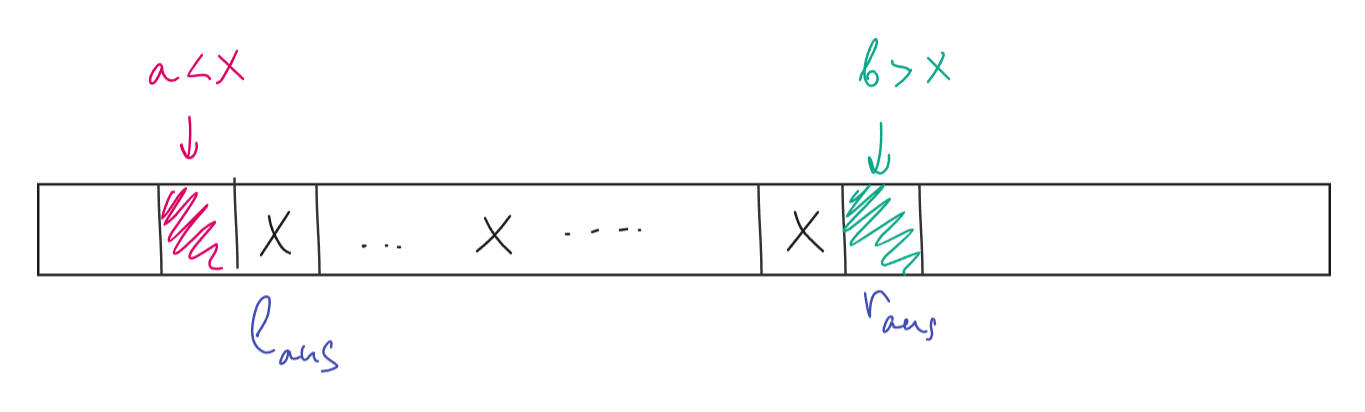
\includegraphics[scale=0.6]{./assets/08-binary-search/1.PNG}
\end{center}


\Subsubsection{STL implementation}

In C++ language we are already provided with the template functions that do the same thing:

\begin{lstlisting}[language=C++]
/* returns iterator (for int* it is a pointer) */
int i = std::lower_bound(a, a + n, x) - a;
int i = std::upper_bound(a, a + n, x) - a;

// For other containers (e.g., std::vector, std::set) that define begin()/end() operations use the following:
std::lower_bound(
    std::begin(container),
    std::end(container),
    element
) //  e.g., for std::vector<T> the return type is std::vector<T>::iterator, i.e. pointer to the element
\end{lstlisting}


\Subsection{Use of a predicate}

We could abstract the implementation even further via searching for a predicate. Predicate is such a function $f: S \to \{0, 1\}$. Then let's consider the predicate $f(i) = if (a_i < x) then 0 else 1$ - in this case the binary search will find such indicies $l$ and $r$ that satisfy the following:

1. $l + 1 = r$

2. $f(l) = 0$ (i.e. $a_l < x$)

3. $f(r) = 1$ (i.e. $a_r >= x$)

\begin{lstlisting}[language=C++]
int binary_search(int l, int r, int x) {
    while(r - l > 1) {
        int m = (l + r) / 2;
        if (f(m)) r = m; // invariant: a[r] >= x
        else l = m; // invariant a[l] < x
    }
    return r;
}

// If you want to parameterize predicate as well:
// #1: provide a 4th argument as a pointer to a function
// (see: https://www.cprogramming.com/tutorial/function-pointers.html)
int binary_search(int l, int r, int x, bool(*f)(int)) {
    ...
}

// #2: template parameter
template<typename /* or class */ Func>
int binary_search(int l, int r, int x, Func f) {
    ...
}
// possible call:
binary_search(l, r, x, []() { /* predicate impl */ });
\end{lstlisting}

\Subsection{Correctness}

You might already noticed that the functions (arrays are also akin functions, i.e. $a: \{0, 1, .., n-1\}: \mathbb{N} $) over which we apply the binary search algorithm are all monotonic functions, i.e. they comply to $x < y: \ f(x) < f(y)$ (strict monotonically increasing functions; the rest are alike).

\begin{lemma}
    \textit{The binary search algorithm over some range [x, y) is correct iff the considered function $f$ is monotonic over [x, y).}
\end{lemma}



\Subsection{Binary search for functions over $\mathbb{R}$}

It is possible to use the binary search with real numbers as well. Let's consider a problem of \textit{finding square root of} $x$:

\underline{\textbf{Problem statement}}: Given $x \in \mathbb{R}$. Find a value $y \in \mathbb{R}$ so that $y^2 == x$ (for us it is $|y^2 - x| < \varepsilon$):

\begin{lstlisting}[language=C++]
double my_sqrt(double x /* never use 'float' */) {
    double l = 0.0;
    double r = x + 1;

    const dobule EPS = 1e-9; // 10^(-9)

    while(r - l > EPS) {
        double m = (r + l) / 2;
        // Preserve invariant: l^2 <= x, r^2 > x
        if (m*m > x) r = m;
        else l = m;
    }

    return (l + r) / 2;
}
\end{lstlisting}

In the above notice: if $0 < y < 1$ then $y^2 < y$, and if $y \geq 1$ then $y^2 \geq 1$. Thus, for $0 < x < 1$ the corresponding $y$ is greater than $x$, i.e. we select $r = x + 1$.

\begin{example} \textbf{Root of a polynomial} $\mathbf{P(x)}$

    Given a polynomial $P(x)$ of \textbf{an odd degree}, i.e. $\deg{P} = 2k + 1$ with the coerfficient for $x^{2k+1}$ be equal to $1$. There exists a root $x_0 \in \mathbb{R}$, and we need to find it.

    \underline{\textbf{Solution}}:

    We could do that using binary search with any precision $\varepsilon$. First, we need to find points $l$ and $r$, such that: $P(l) < 0$ and $P(r) > 0$ (e.g., $l=-\infty, \ r=+\infty$ - \textbf{MAX\_INT} and \textbf{MIN\_INT} in C++):

    \begin{lstlisting}[language=C++]
    for (l = -1; P(l) >= 0; l *= 2);
    for (r = 1 ; P(r) <= 0; r *= 2);
    \end{lstlisting}

    And finally the root search:

    \begin{lstlisting}[language=C++]
        while (r - l > EPS) {
            double m = (l + r) / 2;
            if (P(m) < 0) l = m; // P(l) < 0
            else r = m; // P(r) >= 0
        }
        return (l + r) / 2;
    \end{lstlisting}

    Actually we need exactly $k := \frac{r-l}{\varepsilon}$ iterations, thus the while-loop could be changed by the for-loop.

\end{example}

\Section{Ternary Search}{Vladislav Artiukhov}
\Subsection{Definition, use cases}

Imagine that we need to find a maximum of a function $f(x)$ in the interval $[l, r]$ but now the function is no longer monotonic. Is there a fast way (i.e. as fast as logarithmic asymptotic as in the binary search algorithm) of finding a point $x_0$ such that $f(x_0) \to \max$?

The answer is yes if our function satisfies some constraint.

\begin{definition}
    \textbf{Ternary search algorithm}

    Given a function $f(x)$ and a range $[l, r]$ in which the function is \href{https://en.wikipedia.org/wiki/Unimodality}{\underline{unimodal}} and convex, and we need to find maximum in the range (maximum for convex functions, minimum for concave functions).

    Since the function is unimodal over $[l, r]$ the following holds:

    1. $\forall a, b: l \leq a < b \leq x_0: \ f(a) < f(b)$

    2. $\forall a, b: x_0 \leq a < b \leq r: \ f(a) > f(b)$

    Where $x_0$ is a point where $f(x) = \max$

    \begin{center}
        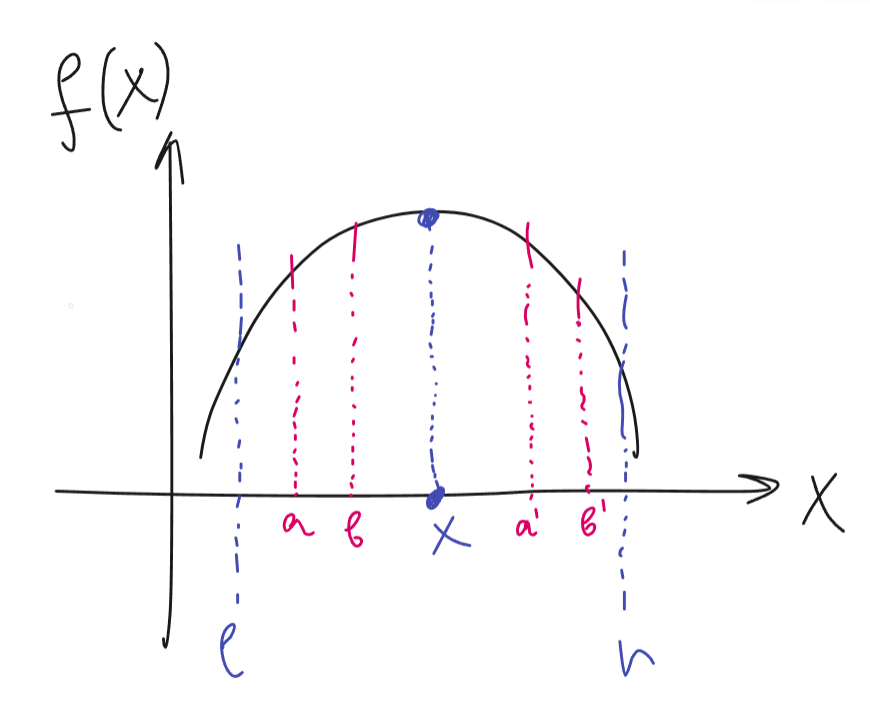
\includegraphics[scale=0.7]{./assets/09-ternary-search/1.PNG}
    \end{center}

    For the algorithm let's consider two points $m_0$ and $m_1$ such that $l < m_0 < m_1 < r$, there are several cases:

    1. $f(m_0) < f(m_1)$, then the maximum of the function $f$ cannot be located in the interval $[l, m_0]$ since there is an interval $[m_0, r]$ on which there are points where function takes greater values.

    2. $f(m_0) > f(m_1)$, then the maximum of the function $f$ cannot be located in the interval $[m_1, r]$ since the interval $[l, m_1]$ contains points in which the function takes greater values.

    3. $f(m_0) = f(m_1)$, in this case the maximum will be located in the interval $[m_0, m_1]$ but for the implementation simplisify this condition branch can be merged with any of the above.

    \begin{center}
        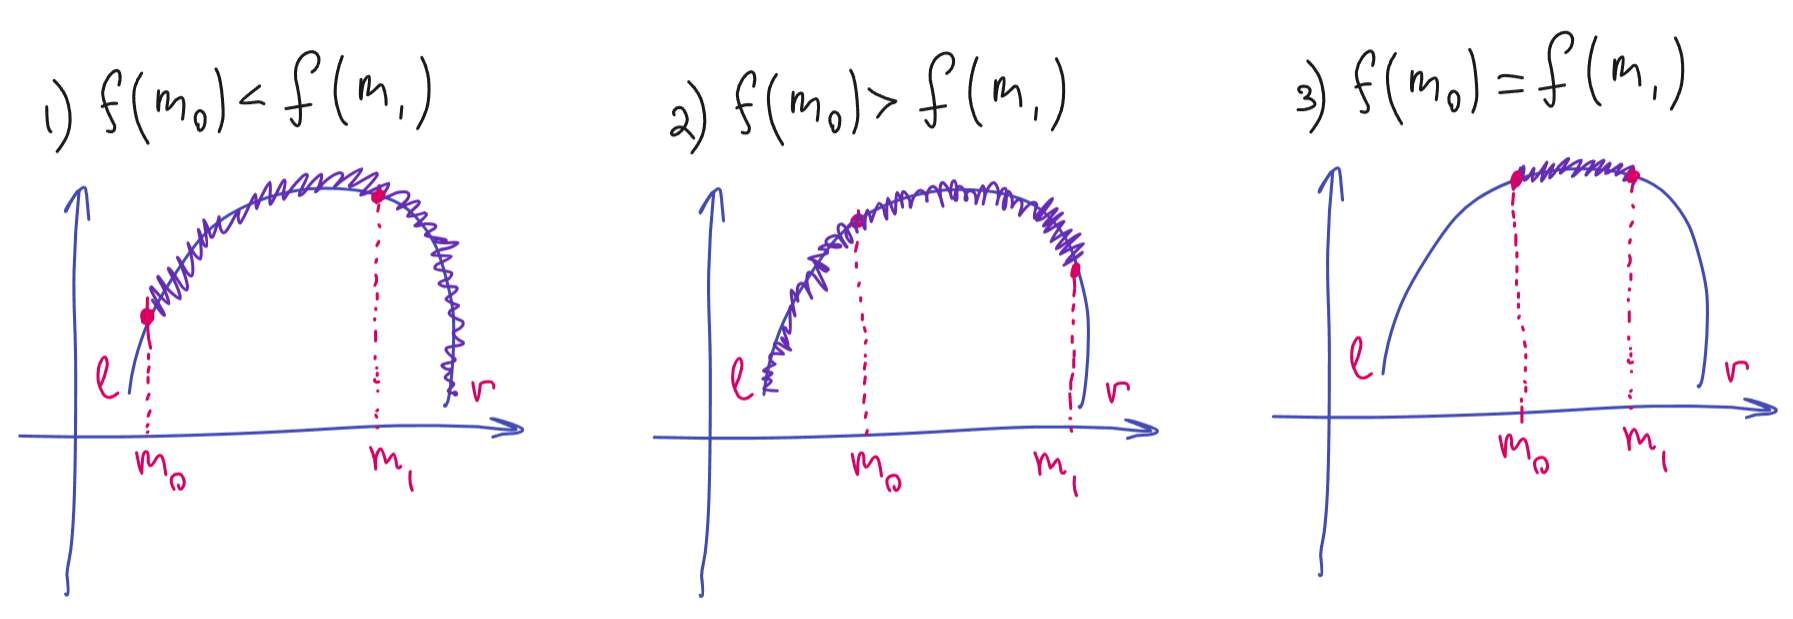
\includegraphics[scale=0.47]{./assets/09-ternary-search/2.PNG}
    \end{center}

    As for the choice of the points $m_0$ and $m_1$ we need to select something that would trancate the remaining searching area in a manner that would give us a logarithmic asymptotic. Let's make $m_0$ be the first 3rd of the interval and $m_1$ be the second 3rd of the interval:

    1. $m_0 = l + \frac{r - l}{3}$

    2. $m_1 = l + 2 \cdot \frac{r - l}{3} = \frac{3l + 2r -2l}{3} = \frac{2r + l}{3} = \frac{3r - r + l}{3} = r - \frac{r - l}{3}$

    Notice that according to the above statement the searching interval becomes $\frac{2}{3}$ of the initial interval, thus:

    $T(n) = T(\frac{2}{3}n) + 1$

    According to \textbf{Master Theorem}:

    $a = 1, \ b = \frac{2}{3}, c = 0, \ f(n) = n^c = 1 \implies a = b^c \implies \Theta(n^c \cdot \log{n}) = \Theta(\log{n}) \implies$

    $T(n) = T(\frac{2}{3}n) + 1 = \Theta(\log{n})$

\end{definition}



\Subsection{Implementation}


Here is the implementation for a function which is an array:

\begin{lstlisting}[language=C++]
int ternary_search(vector<int>& arr) {
    // 'arr' is a unimodal function N -> Z
    int l = 0;
    int r = arr.size();

    while(r - l > 2 /* not 1 because m0 = l, m1 = r possible */) {
        int m0 = l + (r - l) / 3;
        int m1 = r - (r - l) / 3;

        if (arr[m0] < arr[m1]) {
            l = m0;
        }
        else {
            r = m1;
        }
    }

    int ans = l;

    if (r < arr.size() && arr[r] > arr[ans]) {
        ans = r;
    }

    return ans;
}
\end{lstlisting}

Here is the implementation for a function $f$ over floating-point numbers:

\begin{lstlisting}[language=C++]
int ternary_search(double l, double r, double (*f)(double)) {
    while (r - l > EPS) {
        double m0 = l + (r - l) / 3;
        double m1 = r - (r - l) / 3;

        if (f(m0) < f(m1)) {
            l = m0;
        }
        else {
            r = m1;
        }
    }

    return (l + r) / 2;
}
\end{lstlisting}


\Section{Two pointers and Set operations}{Vladislav Artiukhov}
\Subsection{What a set is}

We are going to understand a set as a data structure which contains \textbf{distinct} elements (otherwise \textbf{multiset}) sorted in the \textbf{ascending order}.

STL library contains a data structure that complies to the above definition: \href{https://en.cppreference.com/w/cpp/container/set}{\textbf{std::set<T>}}. In the following subsections we are going to look at fundamental operations over sets. We assume that every time when we are given a set, it is an ascendingly sorted array of distinct elements.

\Subsection{Intersection of sets}

Given two sets $A$ and $B$ and we want to create a set $C = A \cap B$ in $O(|A| + |B|)$:

\begin{lstlisting}[language=C++]
vector<int> intersection(vector<int> A, vector<int> B) {
    int i = 0;
    int j = 0;
    vector<int> C;

    for (; i < |A| && j < |B|; ++j) {
        while (i < |A| && A[i] < B[j]) ++i;
        // last condition means "either 1st element of B or a distinct element"
        // condition can be removed since all elements of bith A and B are distinct
        if (i < |A| && A[i] == B[j] && (j == 0 || B[j - 1] != B[j])) {
            C.push_back(B[j]);
        }
    }

    return C;
}
\end{lstlisting}

The above algorithm can be extended to an intersection of an arbitrary number of sets $A_0, A_1, ..., A_k$. You can try to do that in the following LeetCode problem: \href{https://leetcode.com/problems/intersection-of-multiple-arrays/description/}{2248. Intersection of Multiple Arrays}.



\Subsection{Union of sets}

Given two sets $A$ and $B$, we want to find $C = A \cup B$ in $O(|A| + |B|)$:

\begin{lstlisting}[language=C++]
vector<int> union(vector<int> A, vector<int> B) {
    int i = 0;
    int j = 0;
    vector<int> C;

    for (; j < B.size(); ++j) {
        while (i < A.size() && A[i] <= B[j]) {
            C.push_back(A[i++]);
        }
        // in the case if last added element A[i] is equal to B[j]
        if (C.empty() || C.back() != B[j]) {
            C.push_back(B[j]);
        }
    }

    while (i < A.size()) {
        C.push_back(A[i++]);
    }

    return C;
}
\end{lstlisting}

\Subsection{Difference of sets}

Given two sets $A$ and $B$, we want to find $C = A \setminus B$ in $O(|A| + |B|)$:

\begin{lstlisting}[language=C++]
vector<int> difference(vector<int> A, vector<int> B) {
    int i = 0;
    int j = 0;
    vector<int> C;

    for (; i < A.size(); ++i) {
        // skipping elements less than A[i]
        while(j < B.size() && B[j] < A[i]) {
            ++j;
        }
        // if A[i] not present in B add A[i] to the answer
        if (j >= B.size() || B[j] != A[i]) {
            C.push_back(A[i]);
        }
    }

    return C;
}
\end{lstlisting}

You may solve this task by yourself of LeetCode: \href{https://leetcode.com/problems/find-the-difference-of-two-arrays/description/}{2215. Find the Difference of Two Arrays}

\Subsection{STL implementations}

STL already has implementations of all the operations mentioned above: \href{https://cplusplus.com/reference/algorithm/set\_difference/}{std::set\_difference}, \href{https://cplusplus.com/reference/algorithm/set\_union/}{std::set\_union}, \href{https://cplusplus.com/reference/algorithm/set\_intersection/}{std::set\_intersection}, and \href{https://cplusplus.com/reference/algorithm/merge/}{std::merge} (the latter one is the same as std::set\_union but it does not remove the duplicate elements). All the mentioned STL functions are called in the following manner:

\begin{lstlisting}[language=C++]
int k = std::merge(A, A + |A|, B, B + |B|, C) - C;
// C - pointer to where to store the result (memory allocation is your responsibility)
// k - number of elements in the result, i.e. k == |C|
\end{lstlisting}

\Subsection{Problem example}

% \begin{problem}

%     Given an array $a$ of size $n$ and $m$ queries (all queries are given at once) of type "count the number of distinct numbers in the segment $[l_i, r_i]$ of the array $a$".

%     Time complexity: $O(n + m)$ $O(m \cdot \log{n})$.

%     Space complexity: $O(n + m)$.

% \end{problem}

% \begin{solution}

    % Notice that the problem is an \textbf{offline} task, i.e. all the queries are given, thus we can sort the components $l_i$, $r_i$ in the ascending order $\implies$ now we can treat them us a sequence of \textbf{events} of opening and closing segments.

    % Now we can traverse all the events: every time we encounter $l_i$ we place it in the stack $s$ to later use, once $r_i$ is encountered, due to sorting order, it is the \textbf{closing event} of the opening event $l_i$ on top of the stack $s$

% \end{solution}

\Section{Hash table}{Vladislav Artiukhov}
\Subsection{Hash table with Sliding Window}

\begin{problem}

    Given an integer array $a$ and an integer $k$, return the number of \textbf{good subarrays} of $a$.

    A \textbf{good array} is an array where the number of different (distinct) integers in that array is exactly $k$. A subarray is a \textbf{contiguous part} of an array.

    For example, $[1, 2, 3, 1, 2]$ has $3$ different integers: $1, 2, 3$.

    Asymptotics: $O(n)$ in time and space. \newline


    \underline{Note}: you can solve this problem on LeetCode here \href{https://leetcode.com/problems/subarrays-with-k-different-integers/description/}{992. Subarrays with K Different Integers}.

\end{problem}

\begin{example}

    1. $a = [1,2,1,2,3]$, $k = 2$, the answer will be $7$, the good subarrays are:

    $[1,2], [2,1], [1,2], [2,3], [1,2,1], [2,1,2], [1,2,1,2]$.\newline

    2. $a = [1,2,1,3,4]$, $k = 3$, the answer will be $3$, the good subarrays are:

    $[1,2,1,3], [2,1,3], [1,3,4]$.

\end{example}



\begin{solution}

Idea: $exactly(k) = atMost(k) - atMost(k-1)$, thus let's count the number of subarrays with at most $k$ ($\leq k$) distinct numbers and the number of subarrays with at most $k-1$ distinct numbers.

In order to count distinct numbers if a sliding window we need keep the count of each distinct value in the sliding window.

Once the right border of the window goes forward we increment the count of a new value $a_j$, and if it the count became $1$, then increment $cnt$ (since the number of distinct numbers increased by one).

Once the left border of the window goes forward we decrement the count of a tracked value $a_i$ (before incrementing $i$) and if this value becomes $0$, we decrement the number of distinct values.

Let's keep a sliding window $[i, j]$ that will contain $\leq k$ distinct elements:

1. If current number of distinct values is $\leq k$ we only need to move forward the right boundary $j$ and on each iteration increase the result by $(j - i + 1)$ because the number of subarrays that end in $j$ and contain $\leq k$ distinct values is the number of suffixes the subarray $a[i..j]$ has (suffixes are: $[i+1..j]$, $[i+2..j]$, ..., $[j-1..j]$, $[j..j]$). This way we will count all the subarrays of $a$ that contain $\leq k$ elements.

2. Once the number of distinct values $cnt$ inside the sliding window has become $(k+1)$ we need to move forward the left boundary $i$ until $cnt$ becomes equal to $k$.

By the above algorithm we found the result of the function $atMost(k)$, now do the same for $atMost(k-1)$ and return the their difference.


\begin{lstlisting}[language=C++]
int atMost(vector<int>& nums, int k) {
    unordered_map<int, int> counts;
    int i = 0;
    int cnt = 0;
    int result = 0;

    for (int j = 0; j < nums.size(); ++j) {
        if (counts[nums[j]]++ == 0) {
            ++cnt;
        }

        if (cnt <= k) {
            result += (j - i + 1);
        }

        while (i <= j && cnt > k) {
            --counts[nums[i]];
            if (counts[nums[i]] == 0) {
                --cnt;
            }
            ++i;

            if (cnt == k) {
                result += (j - i + 1);
            }
        }
    }

    return result;
}

int exact(vector<int>& nums, int k) {
    return atMost(k) - atMost(k-1);
}
\end{lstlisting}

\end{solution}

\Section{Binary heap}{Vladislav Artiukhov}
\Subsection{Definition}

Consider an array $a[1..n]$. Its elements form a binary tree with a root at $1$.

Children of a vertex at $i$ are vertices at $2i$ and $2i+1$; the parent of a vertex at $i$ is $\lfloor \frac{i}{2} \rfloor$.

\begin{definition}\textbf{Binary heap}

    A binary heap is an array indicies of which form the described above tree which in turn holds the following property: $\forall$ vertex $i$ the value $a[i]$ is a \textbf{minimum} in a subtree of $i$.

    \begin{center}
        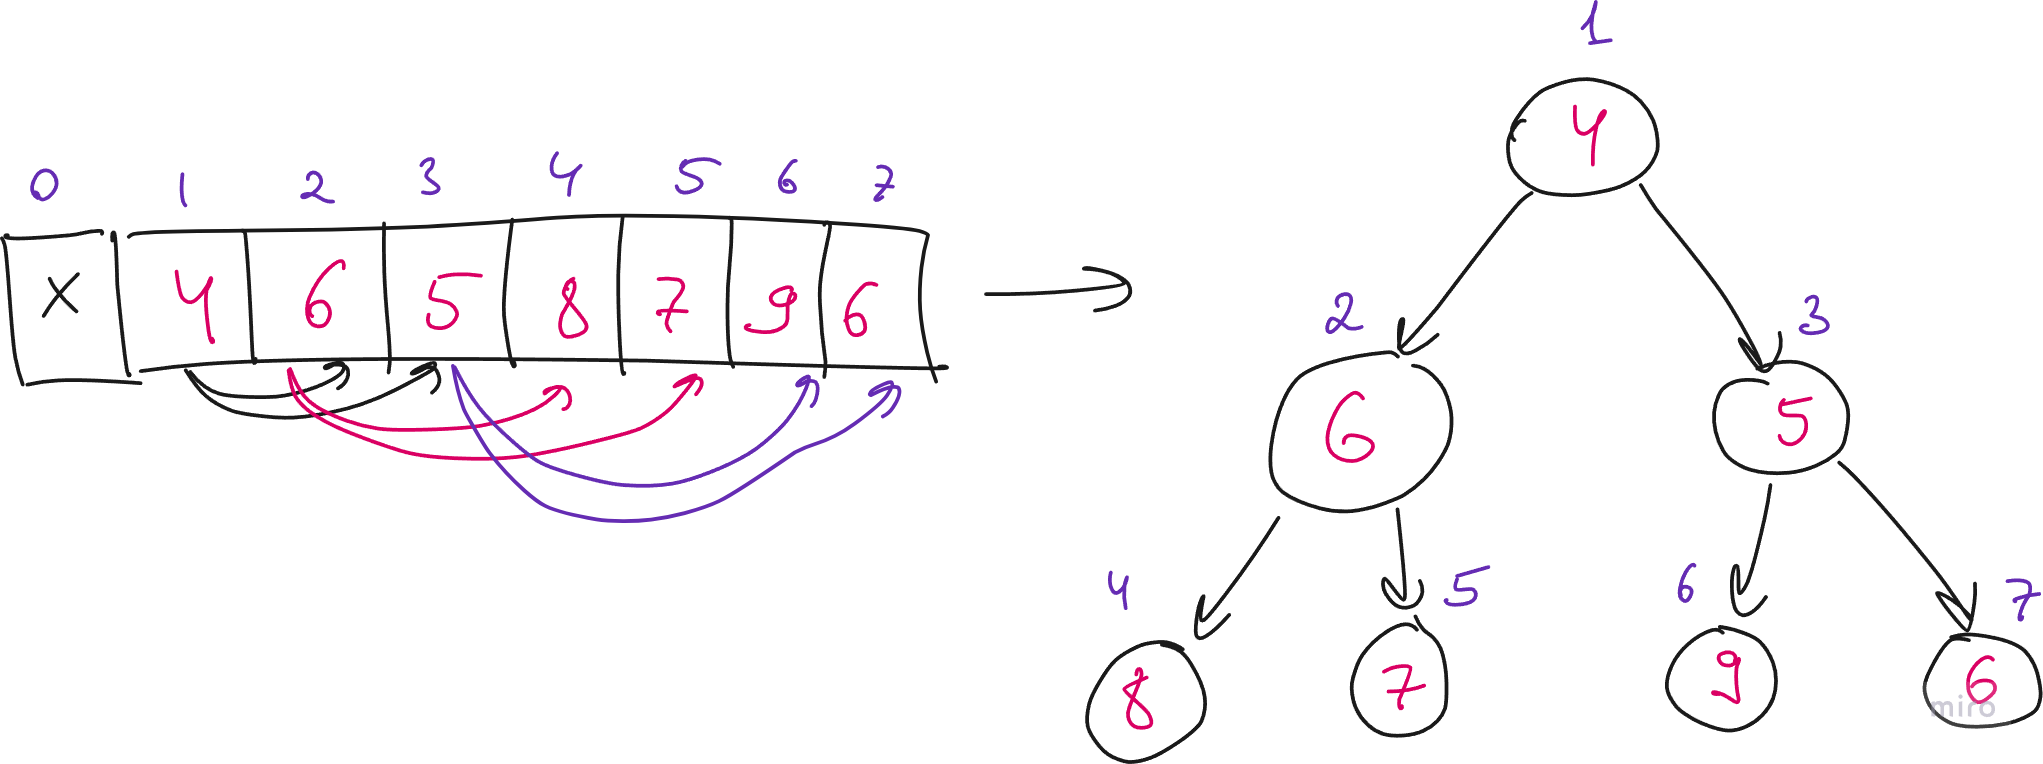
\includegraphics[scale=0.25]{./assets/12-binary-heap/1.png}
    \end{center}

\end{definition}

\begin{lemma}

    The height of the binary heap is $\lfloor \log_{2}{n} \rfloor$.

\end{lemma}

\begin{proof}

    The height is equal to the length of the distance between the vertex at $n$ and the root at $1$. Notice, that by the definition $\forall k$: distance from the root to vertices from the range $[2^k, 2^{k+1})$ is equal to $k$ $\implies$ for the vertex at $n$ its corresponding $k := \lfloor \log_{2}{n} \rfloor$ (it is a simple induction over $k$):

    Let $d_{k}$ be the distance between (in terms of the number of edges) the root and the vertices from the range $[2^k, 2^{k+1})$. We want to prove $d_{k} \equiv k$:

    1. \textbf{Base}: $k=1$

    $[2^1, 2^{2}) = [2, 2^2-1] = [2, 3]$ - distance $d_{1}$ between the root and vertices $2$ and $3$ is indeed $1$ by the definition, thus $d_{1} = k$.

    2. \textbf{Transition:} $k \to k+1$:

    Let's consider the range on the step $k$: $[2^k, 2^{k+1}-1]$, now let's see what are the children for the vertex $v_1 = 2^k$ and the vertex $v_2 = 2^{k+1}-1$ (children of all vertices between $v_1$ and $v_2$ will have numbers in between the obtained range):

        1. $v_1$: $2^k \to 2^{k+1}, 2^{k+1}-1$.

        2. $v_2$: $2^{k+1}-1 \to 2^{k+2}-2, 2^{k+2}-1$.

        Thus, the obtained range will be $[2^{k+1}, 2^{k+2}-1]$, i.e. the distance $d_{k+1}$ from the root to the vertices in this range will be $d_{k+1} = d_{k} + 1 = k+1 \implies d_{k+1} = k+1$.

\end{proof}

\textbf{Interface}:

The binary heap due to its height executes in $O(\log{n})$ the following operations:

1. $GetMin()$ - find the minimum element (works in $O(1)$).

2. $Add(x)$ - add a new element.

3. $ExtractMin()$ - remove the current minimum element.

If there is a support of \textit{reversed references} which allow access to the position $i$ by a given element $a[i]$ in $O(1)$, then the binary heap will also support the following operations:

1. $DecreaseKey(x, c)$ - decrease a value $x$ by $c$.

2. $Del(x)$ - remove element $x$ from the heap.

\Subsection{siftUp, siftDown}

\textbf{siftUp(i)} - push up (bubble up) an element at the position $i$.

\textbf{siftDown(i)} - push down an element at the position $i$.

Both operations require the heap to comply with its definition for all position except the position $i$, i.e. these operations place an element at the position $i$ into such a position, so that the underlying property of a heap starts to hold for all elements.

\begin{lstlisting}[language=C++]
void siftUp(int i) {
    int p = i / 2;
    // while i is not a root and parent's value is greater than value of i
    while (i > 1 && a[p] > a[i]) {
        swap(a[i], a[p]);
        i /= 2;
    }
}

void siftDown(int i) {
    while (true) {
        int l = 2 * i;
        // select a smaller child of i
        if (l + 1 <= n && a[l + 1] < a[l]) ++l;
        // if both children are not less than i
        if (l > n || a[l] >= a[i]) break;
        // go to the child
        swap(a[l], a[i]);
        i = l;
    }
}
\end{lstlisting}

\begin{lemma}

    Both operations work in $O(\log{n})$.

\end{lemma}

\begin{proof}

    Both operations work in $O(\text{heap height}) = O(\log{n})$.

\end{proof}



\Subsection{GetMin, Add, ExtractMin}

All of these operations can be expressed via \textbf{siftUp}/\textbf{siftDown}.

\begin{lstlisting}[language=C++]
vector<int> h(N + 1);
int n = 0; // current size (i.e. the number of elements)

int GetMin() {
    return a[1];
}

void Add(int x) {
    ++n;
    a[n] = x;
    siftUp(n);
}

void ExtractMin() {
    // extracting root
    swap(a[1], a[n]);
    n--;
    siftDown(1);
}
\end{lstlisting}

Example of the \textbf{siftUp} operation during \textbf{Add}:

\begin{center}
    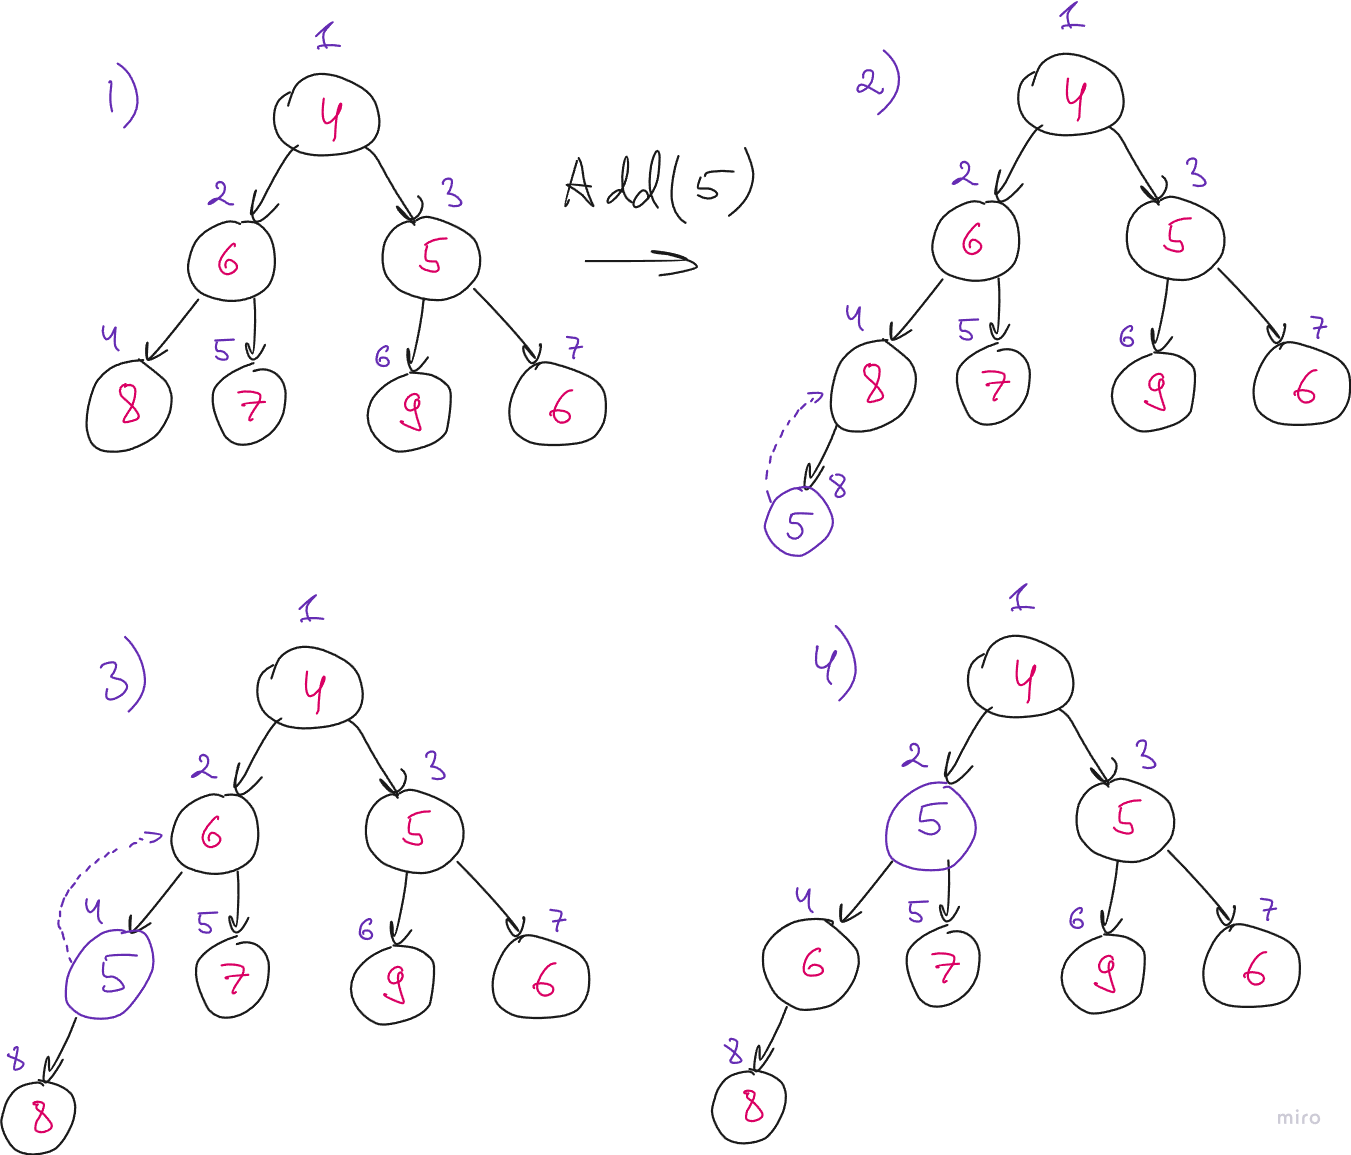
\includegraphics[scale=0.25]{./assets/12-binary-heap/4.png}
\end{center}

Example of the \textbf{siftDown} operation during \textbf{ExtractMin}:

\begin{center}
    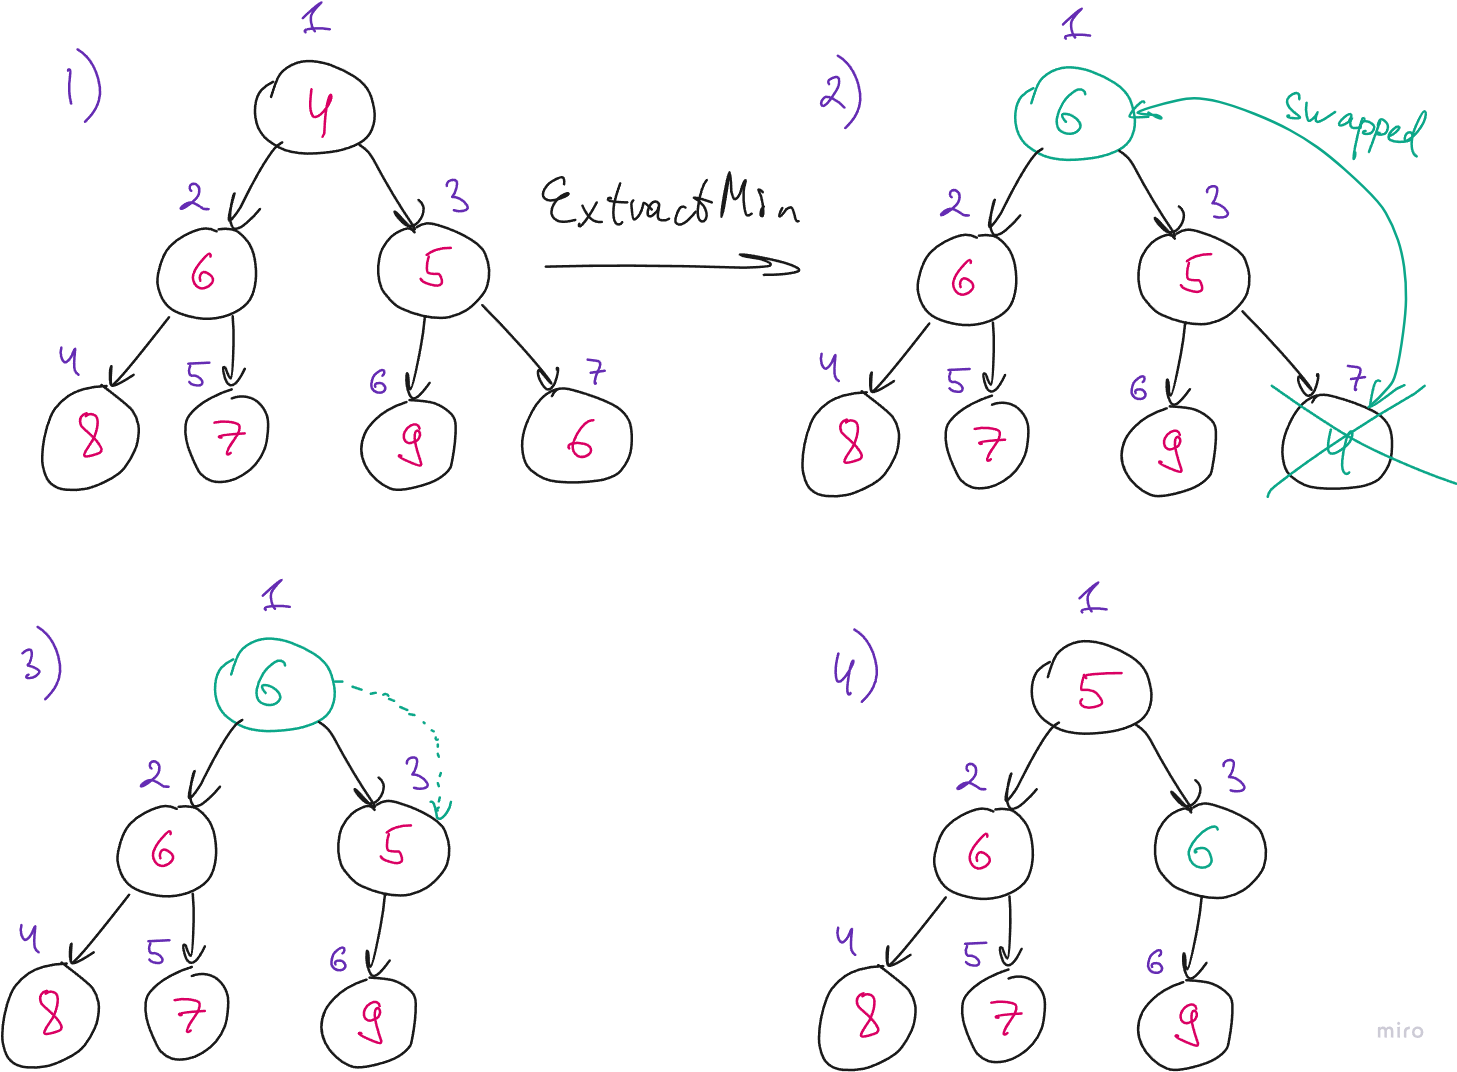
\includegraphics[scale=0.25]{./assets/12-binary-heap/5.png}
\end{center}


\Subsection{Reversed references and DecreaseKey}

Suppose now we have an array \textbf{vector<int> values}. In the heap \textbf{a[]} we will store indicies of the array \textbf{values}. In this case all comparisons $a[i] < a[j]$ will be rewritten as $\text{values}[a[i]] < \text{values}[a[j]]$. In order to add an element we need to add it inside \textbf{values}: \textbf{values.push\_back(x)} and then add its index inside the heap: \textbf{Add(values.size() - 1)}. Since now we store the indicies inside the heap, we can for every $i$ store an index inside the heap, i.e. \textbf{pos[i]} = position of the $i$-th element of \textbf{values} in \textbf{a}.

1. Given position in the heap $\to$ get its value: $i \to a[i] \to \text{values}[a[i]]$.

2. Property of \textbf{pos}: $i \to \text{pos}[i] \to a[\text{pos}[i]] = i$.

The values of \textbf{pos[]} must be recalculated every time when we modify \textbf{a[]}.

See the following image for clarifications:

\begin{center}
    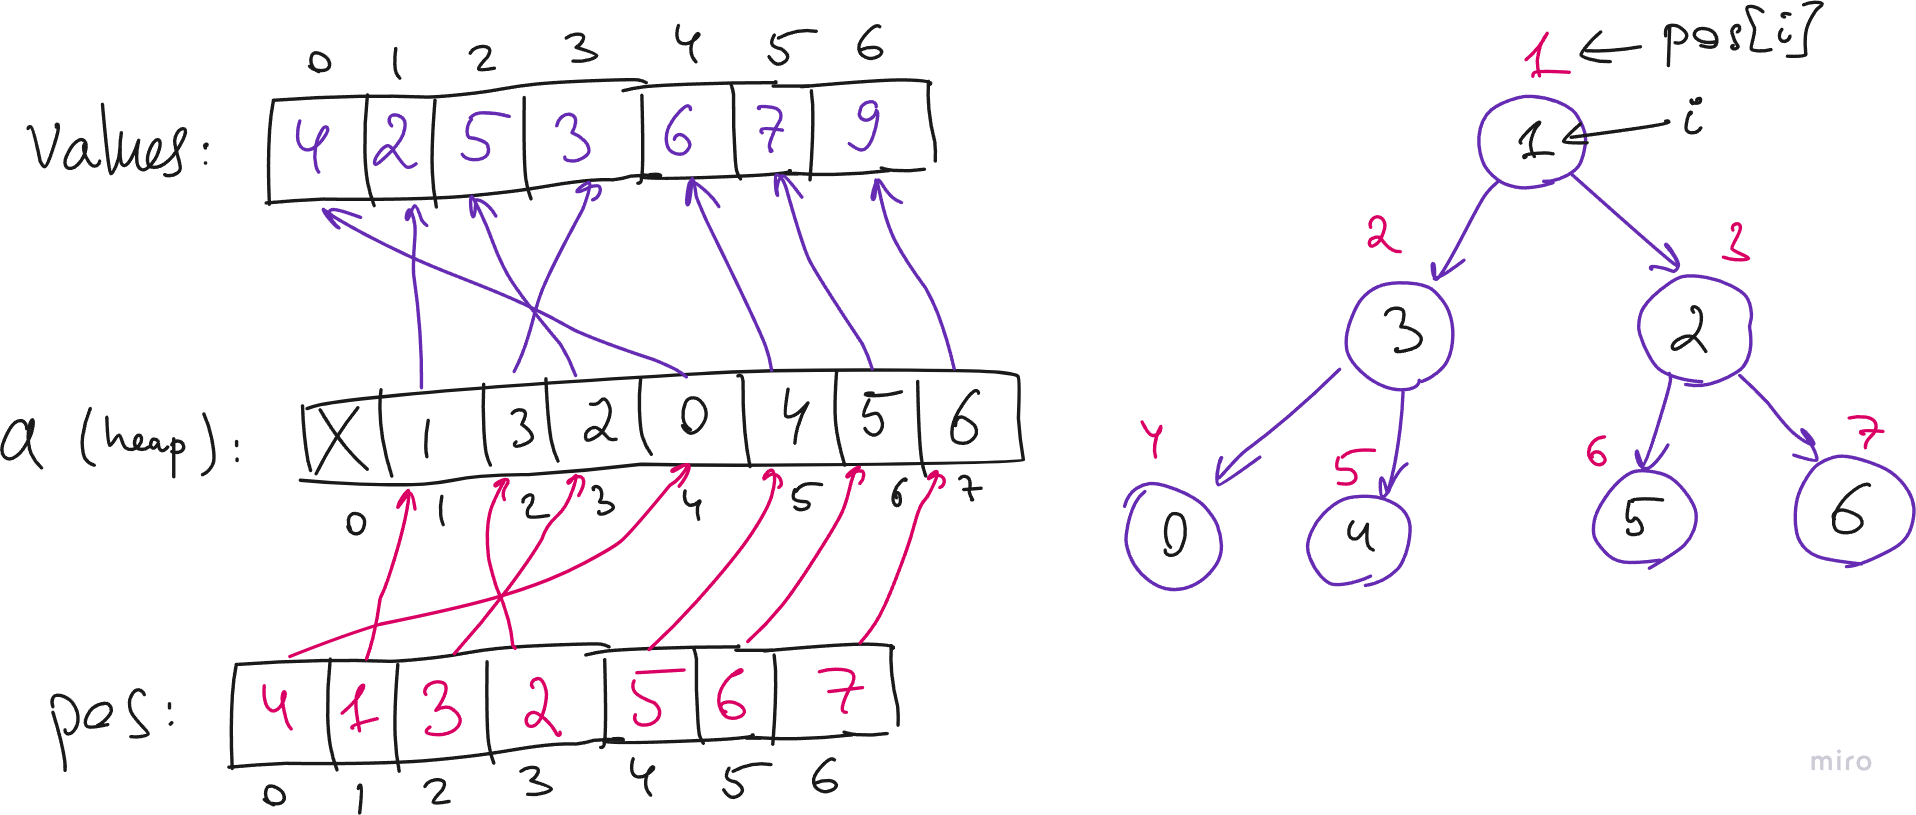
\includegraphics[scale=0.25]{./assets/12-binary-heap/3.png}
\end{center}

Now we can implement removal and decrease of a key of an element inside \textbf{values} by its index $i$ in $O(\log{n})$ of time:

\begin{lstlisting}[language=C++]
void Del(int i) {
    // i - index inside values[]
    int ind = pos[i]; // index inside heap a[]

    a[ind] = h[n]; n--;
    pos[a[ind]] = ind; // update pos[] for the 'a[ind]'-th element of values[]

    // both sift operations because new element can be
    // either greater than its children or less than its parent
    siftUp(ind);
    siftDown(ind);
}

void DecreaseKey(int i, int c) {
    // i - index inside values
    values[i] -= c;
    int ind = pos[i]; // index inside heap a[]

    // the updated element could become less than its parent
    siftUp(ind);
}
\end{lstlisting}


\Subsection{Build, HeapSort}

We can construct a heap from a list of given elements inplace:

\begin{lstlisting}[language=C++]
void Build(int n, int a[]) {
    for (int i = n; i >= 1; --i) {
        siftDown(i);
    }
}
\end{lstlisting}

\begin{lemma}
    The \textbf{Build} operation will construct a correct binary heap from the array \textbf{a[]}.
\end{lemma}

\begin{proof}
    When we push down $i$, due to induction assumption, the left and the right subtrees are already correct binary heaps. Due to correctness of \textbf{siftDown} operation after its execution the subtree at $i$ will become a correct binary heap.
\end{proof}

\begin{lemma}
    \textbf{Build} works in $\Theta(n)$ of time.
\end{lemma}

\begin{proof}
    Let $n = 2^k-1$, then our heap is a full binary tree, because each element except for the leaves will have 2 children. The last level of the heap will contain $2^{k-1}$ elements, the pre-last level will contain $2^{k-2}$ elements, and so on.

    \textbf{siftDown(i)} works in $O(\text{depth of the subtree of $i$})$, thus its total time will be:

    $\sum_{i=1}^{k} 2^{k-i} \cdot i = 2^k \cdot \sum_{i=1}^{k} \frac{i}{2^i} =_{(*)} 2^k \cdot \Theta(1) = (n+1) \cdot \Theta(1) = \Theta(n)$.

    (*): Need to proof that $\sum_{i=1}^{k} \frac{i}{2^i} = \textbf{const}$;

    Notice that $\sum_{i=1}^{k} \frac{i}{2^i} = 2 - \frac{k+2}{2^k}$ (I used \href{https://www.wolframalpha.com/}{wolframalpha} :)). Let's prove it via induction:

    1. \textbf{Base}: $k=1$:

    $\sum_{i=1}^{k} \frac{i}{2^i} = \frac{1}{2} = 2 - \frac{3}{2}$ - the assumption holds.

    2. \textbf{Transition}: $k \to k+1$:

    $\sum_{i=1}^{k+1} \frac{i}{2^i} = \sum_{i=1}^{k} \frac{i}{2^i} + \frac{k+1}{2^{k+1}} = 2 - \frac{k+2}{2^k} + \frac{k+1}{2^{k+1}} = 2 - \frac{k+3}{2^{k+1}} = 2 - \frac{(k+1)+2}{2^{k+1}}$.

\end{proof}

The \textbf{HeapSort} implementation that works in $O(n \log{n})$ and uses $O(1)$ of additional memory due to \textbf{Build} working inplace:

\begin{lstlisting}[language=C++]
void HeapSort(int n, int a[]) {
    Build(n, a);

    for(int i = 0; i < n; ++i) {
        // extracting values in ascending order
        int x = GetMin();
        ExtractMin();
    }
}
\end{lstlisting}


\Section{Sorting Algorithms}{Vladislav Artiukhov}
\Subsection{Basics}

\begin{definition}\textbf{Stable sorting algorithm}

    The given sorting algorithm is called \textbf{stable} if equal elements are placed in the same order (among these equal elements) as it was in the initial placement, i.e. $\forall i \neq j: a_i = a_j, \ \pi$ - some permutation that sorts the elements, then $i < j \implies \pi(i) < \pi(j)$.

\end{definition}

\begin{definition}\textbf{Inversion}

    Inversion is a pair $(i, \ j)$, s.th.: $i < j: a_i > a_j$.
\end{definition}

\begin{definition}
    $I$ - number of inversions in the array.
\end{definition}

\begin{definition}
    The array is sorted $\Leftrightarrow$ $I = 0$.
\end{definition}

\begin{lemma}

    The sorting algorithm $A$ based on the comparisons of the elements which does $o(n \log{n})$ comparisons for all posible inputs of size $n$ is \textbf{incorrect}, i.e. $\exists$ test $T$ on which the result of sorting by $A$ will be \textbf{incorrect}.

\end{lemma}

\begin{proof}

    Notice that an input of size $n$ can be expressed as a permutation of indicies $\pi: I \to I$ where $I$ is the set of indicies, i.e. $I:=\{0, 1, 2, .., n-1\}$, then there exist $n!$ inputs.

    \begin{center}
        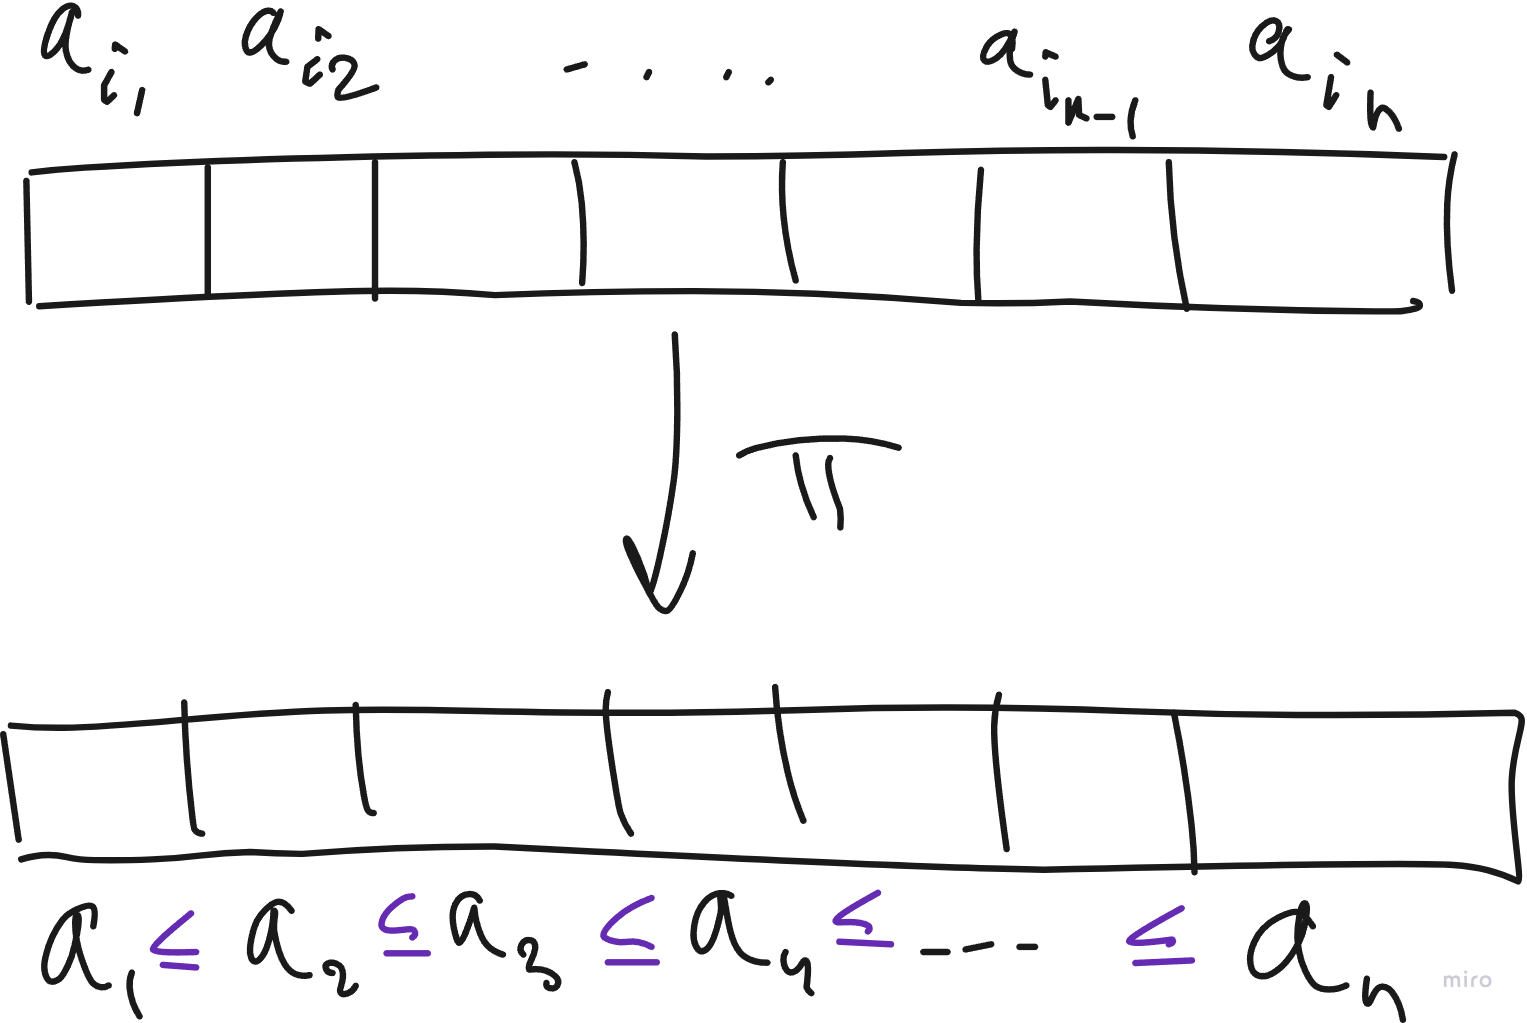
\includegraphics[scale=0.18]{./assets/13-sorting-algorithms/3.png}
    \end{center}

    For the proof it is convinient for us to think that for every input the algorithm $A$ does exactly $k$ comparisons (if in fact it does less then let's just do some meaningless comparisons to get exactly $k$).

    Since the sorting algorithm $A$ is based on comparisons we can assign a binary value for each comparison. The algorithm does $k$ comparisons, if on the $i$-th position the comparison yielded "less or equal" then we assign $0$, if it yielded "greater" we assign $1$ $\implies$ we end up having a binary string of size $k$. Notice that there is a bijection between the set of the produced strings of size $k$ and the set of inputs of size $n$ $\implies$ $2^k = n!$:

    $o(n \log{n}) = \log{2^k} = \log{n!} \implies \log{n!} = o(n \log{n})$ but we know that $\log{n!} = \Theta(n \log{n})$, thus there is a no bijection $\implies$ there exist a test on which the algorithm $A$ produces a wrong result.

\end{proof}


\Subsection{CountSort}

This algorithm sorts a set of integers in range $[0, m)$ in $O(n + m)$ of time and $O(m)$ of memory where $n$ is the size of the input array.

\begin{lstlisting}[language=C++]
int n;
int arr[n];
int count[M] = {0};

for (int i = 0; i < n; ++i) { // O(n)
    count[x]++;
}

for (int x = 0; x < M; ++x) { // O(n + M)
    while(count[x]--) {
        std::cout << x << " ";
    }
}

\end{lstlisting}

Notice that this sorting algorithm is based on the counting not comparisons, thus it is correct and there is a speed boost.


\Subsection{MergeSort: recursive and iterative solutions}

The main idea is to sort the left part, sort the right part and then merge two sorted parts into a single sorted array via two pointers approach.

\Subsubsection{Recursive implementation}

\begin{lstlisting}[language=C++]
void MergeSort(int l, int r, int* a, int* buffer) { // [l, r)
    // base case
    if (r - l <= 1) return;

    int m = (l + r) / 2;
    // sort [l, m)
    MergeSort(l, m, a, buffer);
    // sort [m, r)
    MergeSort(m, r, a, buffer);

    // merge two sorted halves via 2 pointers in O(r - l) time
    Merge(l, m, r, a, buffer);
}
\end{lstlisting}

\textit{buffer} is an additional chunk of memory which is required for the \textbf{Merge} method. The \textbf{Merge} goes through the $[l, m)$ and $[m, r)$ and puts them according to the two pointers technique into the \textit{buffer}.

\begin{lemma}

    Time complexity is $O(n \log{n})$.

\end{lemma}

\begin{proof}
    The recursive formula is as follows: $T(n) = 2 \cdot T(\frac{n}{2}) + n$.

    \underline{Note (Master Theorem)}: $T(n) = a \cdot T(\frac{n}{b}) + n^c$.

    According to the Master Theorem: $a = 2, b = 2, c = 1 \implies a = b^c \implies O(n^c \log{n}) = O(n \log{n})$.

\end{proof}

\Subsubsection{Iterative implementation}

Suppose that the size of the input array is $n = 2^m$ (if not then pad the array with \textbf{MAX\_INT} until it becomes $2^m$). In the recursive approach we traverse the recurse tree from top to bottom, here we traverse it from bottom up. At the bottom we have chunks of size $1$, on the next level chunks of size $2^1$, on the next $2^2$ and so on.

\begin{lstlisting}[language=C++]
int n;
vector<int> arr(n), buffer(n);
// In C++: (1 << k) == 2^k
for (int k = 0; (1 << k) < n; ++k) {
    // iterate through pairs of chunks of size 2^k
    for (int i = 0; i < n; i += 2 * (1 << k)) {
        int m = min(n, i + (1 << k));
        int r = min(n, i + 2 * (1 << k));
        Merge(i, m, r, arr, buffer);
    }
    // now buffer has properly sorted chunks of size 2^(k+1),
    // we need arr to store the updated result after each iteration.
    swap(arr, buffer); // O(1)
}
// the answer is here because we always updated arr inside the for-loop
return arr;

\end{lstlisting}

\begin{center}
    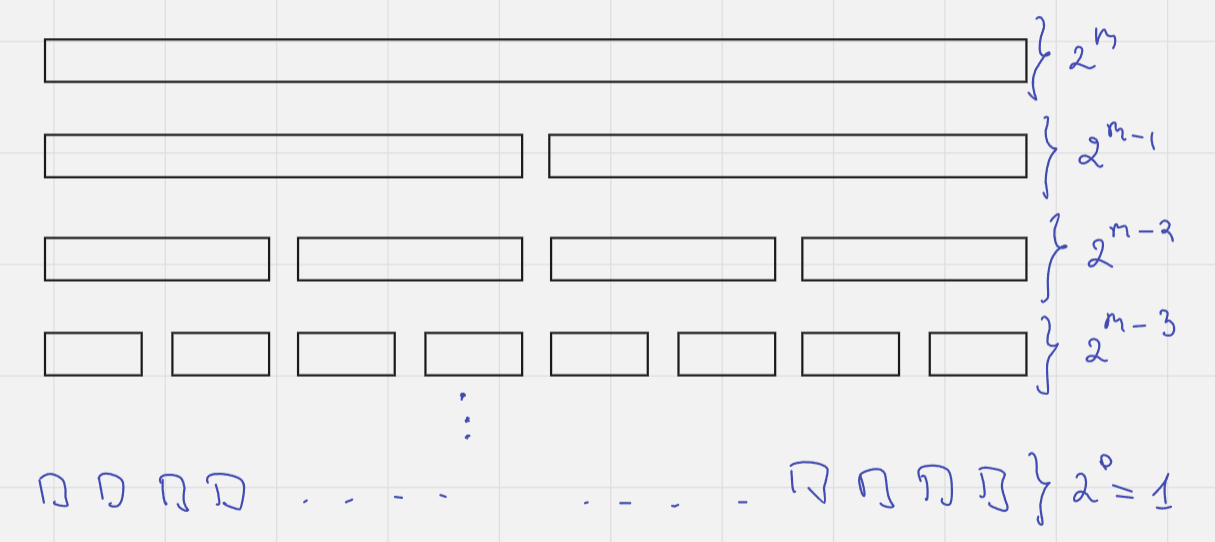
\includegraphics[scale=0.6]{./assets/13-sorting-algorithms/1.PNG}
\end{center}

\Subsection{QuickSort}

\underline{The idea:} select an $x$, split the given array $a$ into 3 parts: $<x$, $=x$, $>x$, then make 2 recursive calls to sort the 1st and the 3rd parts.

\begin{lstlisting}[language=Python]
def QuickSort(a):
    if len(a) <= 1: return a
    x = random.choice(a)
    p1 = select (< x)
    p2 = select (= x)
    p3 = select (> x)
    return QuickSort(p1) + p2 + QuickSort(p3)
\end{lstlisting}

The above is the general idea of the algorithm. In order to make it practically quick the following strategy is used to split the array into 3 parts:

\begin{lstlisting}[language=C++]
void partition(int l, int r, int x, int* a, int &i, int &j) { // [l, r] - both inclusive
    assert(x in a[l..r]); // x must be from a
    i = l;
    j = r;
    while(i <= j) {
        while (a[i] < x) i++;
        while (a[j] > x) j--;
        // a[i] >= x, a[j] <= x => swap elements
        if (i <= j) swap(a[i++], a[j--]);
    }
}
\end{lstlisting}

The above \textit{partition} will split the array into 3 parts $[l, j](j, i)[i, r]$ where:

1. $a[l, j] \leq x$.

2. $a[j+1, i-1] = x$.

3. $a[i, r] \geq x$.

\begin{lemma}
    The algorithm will not exceed the bounds $[l, r]$.
\end{lemma}

\begin{proof}
    $x \in a[l, r] \implies$ there will be at least one \textbf{swap} operation executed (e.g. once $a[i] = x$ and $a[j] = x$). After the last \textbf{swap} the following holds: $l \leq i,\ i \geq j,\ j \leq r$.
\end{proof}

The implementation of the \textbf{QuickSort}:

\begin{lstlisting}[language=C++]
void QuickSort(int l, int r, int* a) { // [l, r] - both inclusive
    if (l >= r) return;
    int i, j;
    int x = a[random in [l, r]];
    // partition accepts i and j by reference and updates them
    Partition(l, r, x, i, j);
    // now: a[l,j] < x, a(j, i) = x, a[i, r] > x
    // we need to sort the 1st and the 3rd parts
    QuickSort(l, j, a); // j < i
    QuickSort(i, r, a); // j < i
}
\end{lstlisting}

\Subsection{Comparison of the sorting algorithms}

\begin{center}
    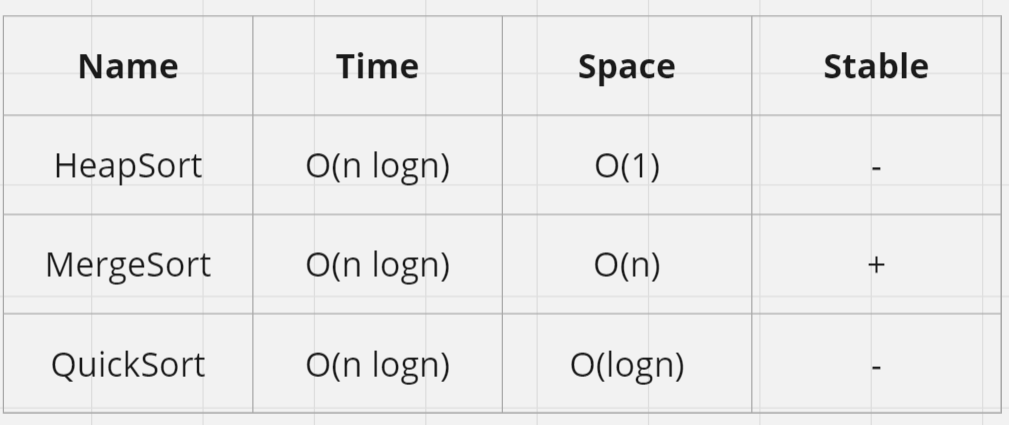
\includegraphics[scale=0.6]{./assets/13-sorting-algorithms/2.PNG}
\end{center}

Notice that among the mentioned sorting algorithms no one is able to make a stable sorting in $O(1)$ of space. There exist such an algorithm, it is implemented via \textbf{inplace stable merge} in $O(n \log{n})$ of time and $O(1)$ of space.

\Subsection{Integer Sorting}

\Subsubsection{Stable CountSort}

Let's take a look at somewhat altered sorting problem: we are given an array of pairs $(a_i,\ b_i)$ of integers and we need to sort in a \textbf{stable} manner.

\begin{lstlisting}[language=C++]
int pos[n] = {0};
int count[m] = {0};

void CountSort(int n, int* a, int* b) { // 0 <= a[i] < m
    for (int i = 0; i < n; ++i) {
        // count the number of occurrences of a[i]
        count[a[i]]++;
    }

    // pos[i] = "position of the start of the chunk which contains pairs <i, ?>"
    pos[0] = 0;
    for (int i = 0; i + 1 < m; ++i) {
        pos[i + 1] = pos[i] + count[i];
    }
    for (int i = 0; i < n; ++i) {
        int index = pos[a[i]]++;
        result[index] = {a[i], b[i]};
    }
}
\end{lstlisting}

Since the algorithm is \textbf{stable} the following algorithm in the next section can be implemented.


\Subsubsection{RadixSort}

Let's sort $n$ strings of length $L$ where symbols of strings are integers in range $[0, k)$.

\textbf{Algorithm}: firstly, sort (via stable sorting algorithm) by the \textbf{last} symbol, then sort by the pre-last symbol, .., sort by the 1st symbol.

\textbf{Correctness}: we are sorting via a stable sorting algorithm some strings by a symbol on the position $i$. In this case, the strings are already sorted by the suffix $(i, L]$. Due to stability of the sorting algorithm, we can state that the strings that have equal $i$-th symbols will be sorted preserving their relative order after previous sorting iteratation, i.e. by the suffix $(i, L]$ $\implies$ the strings are now sorted by suffix $[i, L]$.

\textbf{Time complexity}: $L$ times we call the \textbf{CountSort} algorithm $\implies$ it will sort the strings in $\Theta(L \cdot (n + k))$.

Notice that $\forall b$ - the integer system base, any integer in $[0, m)$ is a string of length $\log_{b}{m}$ over the alphabet $[0, b) \implies$ we can sort integers over base $b$ in $\Theta((n + b) \cdot \lceil \log_{b}{m} \rceil)$. Then once $b = n$ we have the optimum time of $\Theta(n \cdot \lceil \log_{n}{m} \rceil)$.

\underline{The idea of the integer sorting}: we transform integers of the given array from the base of $10$ into the base of $n$ and apply the string sorting algorithm described above.


\Subsubsection{BucketSort}

The idea is to place all of the elements $x$ ($\min \leq x \leq \max$) into $n$ buckets. In order to do that the numeric line is splitted into $n$ segments of equal size where the $i$-th segment contains the elements from the following range:

$L := \max - \min + 1$, $[\min + \frac{i}{n}L, \ \min + \frac{(i+1)}{n}L)$

In this case, each element $x_j$ will be placed into the segment of number $i_j = \lfloor \frac{x_j - \min}{L} \cdot n \rfloor$. The buckets themselves are already sorted, we only need to sort elements inside each bucket. It can be done either by calling the BucketSort recursively or by running any other integer sorting algorithm on each bucket.

\begin{lstlisting}[language=C++]
void BucketSort(vector<int>& a) { // we update the provided array
    if (a.empty()) return;
    int n = a.size();
    int min = min_element(a);
    int max = max_element(a);
    int L = max - min + 1;

    if (min == max) return;
    vector<int> buckets[n]; // array of n vectors

    for (int x : a) {
        int bucketIndex = n * (x - min) / L;
        buckets[bucketIndex].push_back(x);
    }
    a.clear();
    for (int i = 0; i < n; ++i) {
        // sort the i-th bucket
        BucketSort(buckets[i]);
        // place the elements back into a
        for (int x : buckets[i]) {
            a.push_back(x);
        }
    }
}
\end{lstlisting}

\begin{lemma}
    BucketSort works in $O(n \cdot \lceil \log{(\max - \min)} \rceil)$ of time.
\end{lemma}

\begin{proof}
    The algorithm divides the numbers into buckets only if $n \geq 2$, thus the $L$ is being reduced on each recursive call at least by $2$ (in particular, $L \to \frac{L}{n}$) $\implies$ the depth of the recursion is not more than $\log{L}$, each recursion level has not more than $n$ buckets.
\end{proof}

\end{document}